%==============================================================
This chapter describes the history of MCS-4 system.
%==============================================================
\section{The Birth of the World's First Microcomputer}
Minicomputers were built using multiple IC chips to construct the processor (CPU). However, in 1971, the year following the release of the historically significant PDP-11, the world’s first single chip microprocessor, the 4004 was born. This section provides an overview of its development. A Japanese engineers played a significant role in making this breakthrough a reality.\cite{4004_Shima}

%==============================================================
\section{Calculators Built with Discrete Components}
From the 1960s to the 1970s, calculator manufacturers around the world fiercely competed to develop new products. Initially, these machines were assembled using discrete components such as TTL ICs, and their logic circuits were entirely constructed using combinational logic. However, as customer demands prompted frequent specification changes, manufacturers began shifting to a stored program approach that embedded macro instructions into ROM like circuits and processed operations sequentially. This architectural transition laid the groundwork for what would eventually become microcomputers. That said, each of these macro instructions represented a large, calculator specific function. Fetching a single instruction typically invoked a substantial sequence (such as waiting for key input, printing on paper, or performing multi digit addition).

%==============================================================
\section{The Move Toward LSI Integration}
In 1969, the same year Apollo 11 landed humans on the moon, Sharp announced the QT-8D, the world’s first eight-digit calculator using MOS LSI technology. Developed in collaboration with Rockwell in the U.S., this four chip configuration achieved both significantly reduced power consumption and a dramatic drop in component count. From this point on, many calculator makers began shifting their focus toward LSI development.

%==============================================================
\section{Busicom's Initiative}
Busicom Corporation was one of Japan's prominent calculator manufacturers at the time. In 1969, Busicom began exploring LSI development for calculators and chose Intel, a U.S. company that specialized in producing LSI using the PMOS process, as a development partner. At the time, Intel was primarily a memory company, manufacturing DRAM and PROM.

%==============================================================
\section{The Birth of the Microcomputer Concept}
The leading figure behind calculator LSI development at Busicom was Masatoshi Shima, a Japanese engineer. In June 1969, he traveled to the U.S. and initiated discussions on calculator LSI specifications at Intel. Initially, the idea was to implement calculator functions using macro instructions specific to calculators. However, the growing complexity of the LSI led to concerns about cost. At one point, Intel engineers proposed abandoning macro instructions in favor of microinstructions. These were simpler and more general purpose than calculator specific macros, closely resembling the instructions used in modern microcomputer CPUs This proposal drastically simplified the hardware, making it a cost effective solution. Thus, the idea of a 4-bit CPU, the 4004, as a microcomputer architecture was born (Figure~\ref{fig:Outline_4004}). Although general purpose CPUs already existed in the form of minicomputers like DEC's PDP-8, it is likely that without the intense technical discussions between Busicom and Intel around macro instruction systems, the concept of an LSI based microcomputer (i.e., a 4-bit CPU) would never have emerged.

%==============================================================
\section{Development of the MCS-4 System}
To realize Busicom's envisioned calculator system, development expanded beyond the 4004 CPU to include the 4001 ROM, 4002 RAM, and 4003 shift register (Figure~\ref{fig:MCS4CHIPSET}). Design efforts for these chips took into account the 16 pin DIP packaging standard from Intel's DRAM products. By December 1969, the overall specifications were largely finalized. Next came the actual LSI design phase. As the client, Shima himself was incorporated into the team as a logic designer and participated directly in development. Samples of the 4001 and 4003 were completed in October 1970, followed by the 4002 in November, and finally the 4004 in March 1971. Fabricated using a 10μm PMOS process, the 4004 packed 2,300 transistors (roughly equivalent to 600 gates) into a 2mm x 3mm chip (Figure~\ref{fig:DieShot_4004}). Its operating frequency was 740 kHz.

%-------------------------------------------------------------------------
\begin{figure}
    %\centering
    %----Left Figure---------------------------------
    \begin{minipage}{0.65\linewidth}
        %\centering
        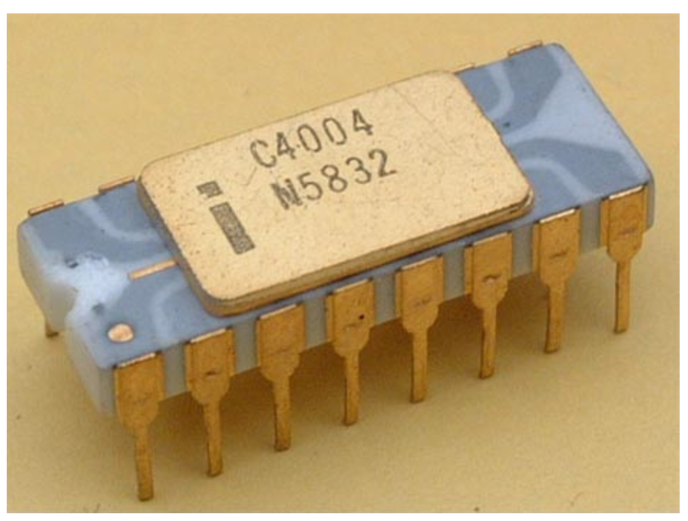
\includegraphics[width=1.0\columnwidth]{./Figure/Outline_4004.png}
        \caption[The world’s first microprocessor: the 4004]{The world’s first microprocessor: the 4004\protect\footnotemark[1]}
        \label{fig:Outline_4004}
    \end{minipage}
    %-------------------------------------------------
    \hspace{0.05\columnwidth}
    %----Right Figure---------------------------------
    \begin{minipage}{0.35\linewidth}
        %\centering
    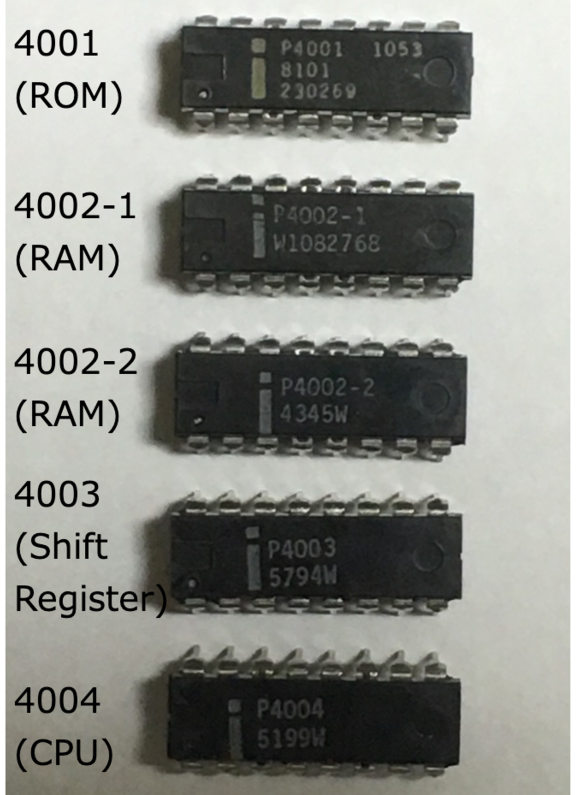
\includegraphics[width=1.0\columnwidth]{./Figure/Outline_MCS4Chipset.png}
    \caption{MCS-4 Chip Set\protect\footnotemark[2]}
    \label{fig:MCS4CHIPSET}
    \end{minipage}
\end{figure}
%-------------------------------------------------------------------------
\footnotetext[1]{Source: \url{http://www.intel-vintage.info/intelmcs.htm}}
\footnotetext[2]{Owned by the author.}

%----------------------------------
\begin{figure}
    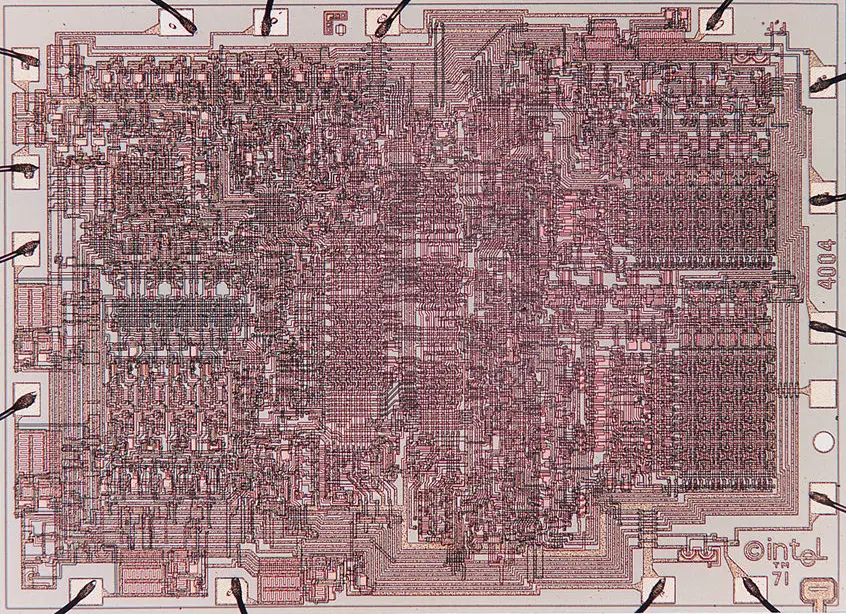
\includegraphics[width=1.0\columnwidth]{./Figure/DieShot_4004.png}
    \caption{Die Photo of the 4004 chip\protect\footnotemark[3]}
    \label{fig:DieShot_4004}
\end{figure}
%----------------------------------
\footnotetext[3]{Source: \url{(https://en.wikichip.org/wiki/intel/mcs-4/4004}}

%==============================================================
\section{The Birth of the Busicom 141-PF Calculator Powered by the Microcomputer}
By April 1971, all the chips had been mounted on the calculator's circuit board, and astonishingly, the system worked perfectly on the first try. This calculator (Figure~\ref{fig:CALC141PF}), released as the 141-PF in 1972, was a 15-digit model with a two color printer. It was already complete as a calculator product, featuring memory functions, percent calculations, and optional square root operations.

%----------------------------------
\begin{figure}
    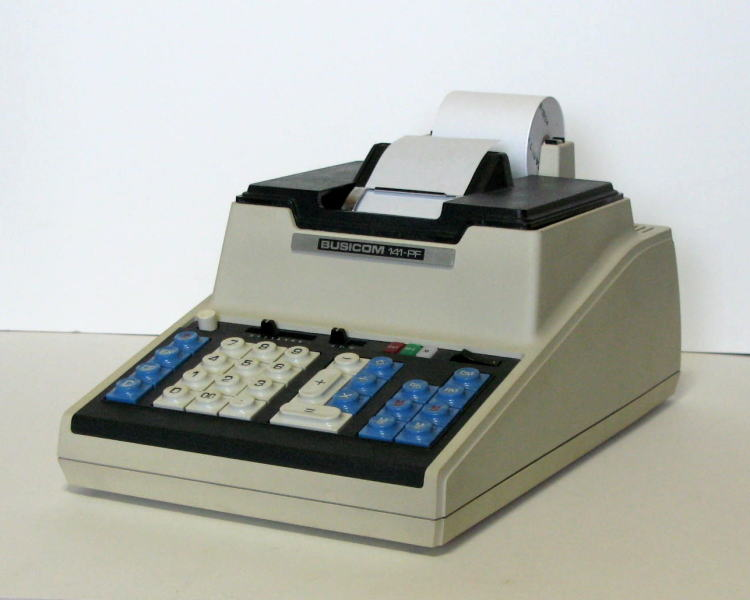
\includegraphics[width=0.75\columnwidth]{./Figure/Busicom_141-PF.png}
    \caption{Busicom's 141-PF Calculator\protect\footnotemark[4]}
    \label{fig:CALC141PF}
\end{figure}
%----------------------------------
\footnotetext[4]{Source: Dentaku-Museum — \url{http://www.dentaku-museum.com/calc/calc/10-busicom/busicomd/busicomd.html}}

%==============================================================
\section{Intel’s Visionary Move}
Initially, the 4001–4004 chipset was developed as a custom product exclusively for Busicom. However, recognizing the general purpose potential of the chips, and aligning with Busicom’s need for capital, Intel renegotiated the contract, returning part of the payment in exchange for the right to sell the chips independently. Intel branded the chip set as the MCS-4 (Micro Computer Set-4) and began sales in November 1971. This marked the beginning of Intel's journey as a CPU manufacturer.

%==============================================================
\section{Japan's Contribution to the Birth of Microcomputers}
Shima's role in the context of calculator application development was extremely significant. Among the many engineers involved in the joint Busicom–Intel project, his contributions to the motivation behind conceiving a general-purpose microcomputer are especially noteworthy. At a time when LSI design tools were nonexistent, logical circuits had to be painstakingly drawn by hand at the transistor level. The excellence of technical execution and the determination to complete a comprehensive system, including the calculator application itself, were truly remarkable.

%==============================================================
\section{Where to See the Intel 4004 and Busicom 141-PF Today}
You can view the actual Intel 4004 and Busicom 141-PF units at the Intel Museum in Silicon Valley, U.S.A (Figure~\ref{fig:INTELMUSEUM}).

%----------------------------------
\begin{figure}
    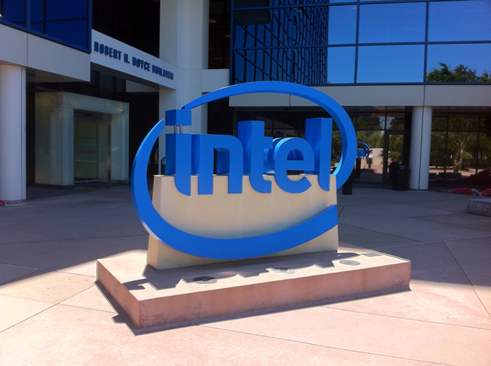
\includegraphics[width=0.5\columnwidth]{./Figure/IntelMuseum.png}
    \caption{ Intel Museum (California, Santa Clara)\protect\footnotemark[5]}
    \label{fig:INTELMUSEUM}
\end{figure}
%----------------------------------
\footnotetext[5]{The author visited here in July 2011.}

%==============================================================
\section{From 4-bit to 8-bit CPUs and Beyond}
Decimal based calculators naturally paired well with 4-bit CPUs like the 4004. However, as systems started handling characters (e.g., ASCII), 8-bit processing became necessary. Following the 4004, Intel developed the 8008 and 8080, the 8- bit CPUs that went on to become major commercial successes. The author recalls being captivated by the charm of microcomputers through NEC’s TK-80 single-board kit (Figure~\ref{fig:TK80}), which featured the 8080A (an enhanced version of the original 8080 with improved drive strength). From there, microcomputing evolved rapidly from 16-bit to 64-bit CPUs and ever more powerful architectures. The pace of progress, as we now know, has been astounding.

%----------------------------------
\begin{figure}
    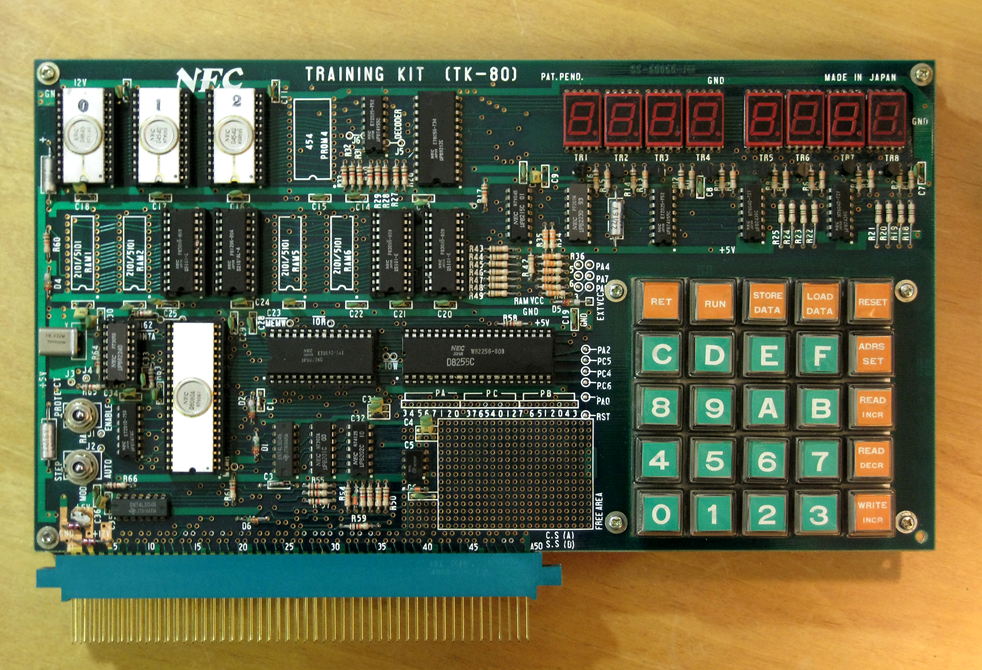
\includegraphics[width=0.5\columnwidth]{./Figure/TK-80.png}
    \caption{NEC’s TK-80 single-board kit\protect\footnotemark[6]}
    \label{fig:TK80}
\end{figure}
%----------------------------------
\footnotetext[6]{ \url{https://en.wikipedia.org/wiki/TK-80}}

%===============================================================================




